\documentclass[a4paper, 11pt]{article}
\usepackage[swedish]{babel}
\usepackage{hyperref}
\usepackage[margin=0.5in]{geometry}

\usepackage{amsmath}
\usepackage{siunitx}
\usepackage[arrowdel]{physics}

\renewcommand{\C}{\mathcal{C}}
\renewcommand{\S}{\mathcal{S}}
\newcommand{\V}{\mathcal{V}}
\newcommand{\rey}{\mathcal{R}}
\newcommand{\erfc}{\text{erfc}}
\newcommand{\ub}[1]{\vb{e}_{\vb{#1}}}
\newcommand{\cha}[1]{\delta #1}
\newcommand{\del}[3][]{\partial_{#2}^{#1}#3}
\newcommand{\mdv}[2][]{\dv[#1]{#2}{t}}
\newcommand{\integ}[5][]{\int\limits_{#2}^{#3}\dd[#1]{#4}#5}
\newcommand{\vinteg}[4]{\int\limits_{#1}^{#2}\dd{\vb{#3}}\cdot #4}
\newcommand{\tinteg}[4]{\int\limits_{#1}^{#2}\dd{\vb{#3}}\times #4}

\title{Sammanfattning av SG1218 Strömningsmekanik}
\author{Yashar Honarmandi \\ yasharh@kth.se}
\date{\today}

\begin{document}

\maketitle

\begin{abstract}
	Detta ær en sammanfattning av kursen SH1014 Modern fysik.
\end{abstract}

\pagenumbering{roman}
\thispagestyle{empty}

\newpage

\tableofcontents

\newpage

\pagenumbering{arabic}

\section{Notation}
Om inte annat specifieras, kommer alla ekvationer använda notationen som ges i denna tabellen.

\begin{table}[!h]
	\centering
	\begin{tabular}{| l | c |}
		\hline
		\textbf{Storhet} & \multicolumn{1}{|l|}{\textbf{Symbol}}\\
		Position         & $\vect{r}$ \\
		\hline
		Tid              & $t$ \\
		\hline
		Period           & $T$ \\
		\hline
		Frekvens         & $f$ \\
		\hline
		Vinkelfrekvens   & $\omega$ \\
		\hline
		Våglängd         & $\lambda$ \\
		\hline
		Vågvektor        & $\vect{k}$ \\
		\hline
		Vågtal           & $k$ \\
		\hline
		Amplitud         & $A$ \\
		\hline
		Vågfart          & $c$ \\
		\hline
	\end{tabular}
\end{table}

\section{Vektoranalys}

Vi kommer här demonstrera lite grundläggande vektoranalys för kontinua som flödar. Mer specifikt kommer vi demonstrera hur flödet påverkar hur man gör integraler i såna kontinua.

\paragraph{Hastighetsfältet}
Hastighetsfältet $\vb{u}$ är ett vektorfält som anger i vilken riktning och hur snabbt ett kontinuum flödar. Vi betecknar i bland dets komponenter som $u, v, w$.

\paragraph{Tidsändring och materiell derivata}
Betrakta ett volymselement. Om det vid en given tid befinner sig i $\vb{r}$, kommer det under en tid $\cha{t}$ förflytta sig en sträcka $\cha{\vb{r}}$. Värdet av något fält $\phi$ i det fluidelementet kommer då vara
\begin{align*}
	\phi(\vb{r} + \cha{\vb{r}}, t + \cha{t}) = \phi(\vb{r}, t) + \del{t}{\phi}\cha{t} + \del{i}{\phi}\cha{x_{i}}.
\end{align*}
Den totala tidsderivatan av $\phi$ för det givna elementet fås genom att beräkna ändringen av fältet och dela på den lilla tidsskillnaden. Vi får då
\begin{align*}
	\dv{\phi}{t} = \del{t}{\phi} + \del{i}{\phi}\frac{\cha{x_{i}}}{\cha{t}} = \del{t}{\phi} + \del{i}{\phi}u_{i} = \del{t}{\phi} + (\vb{u}\cdot\grad)\phi.
\end{align*}
Detta kallar vi för den materiella derivatan av $\phi$.

\paragraph{Tidsderivator av integraler}
Det gäller att
\begin{align*}
	\dv{t}\integ{V}{}{V}{\phi}   &= \integ{V}{}{V}{\del{t}{\phi}}, \\
	\dv{t}\integ{\V}{}{\V}{\phi} &= \integ{\V}{}{\V}{\del{t}{\phi}} + \vinteg{\mathcal{S}}{}{\mathcal{S}}{\phi\vb{u}} = \integ{\V}{}{\V}{\del{t}{\phi} + \div(\phi\vb{u})}.
\end{align*}

\section{Grundläggande koncept}

\paragraph{Syftet med reglerteknik}
Reglerteknik handlar om att kontrollera olika storheter, ofta betecknad $y$, i ett system mot något värde, ofta betecknad $r$. I tillägg till systemets egna beteende påverkas storheten vi vill reglera typiskt av en yttre störning $v$. Vi kan reglera systemet genom att tillföra en påverkan, ofta betecknad $u$.

\paragraph{Strategi}
För att förstå systemet, tar vi först fram en modell som beskriver det. Ur denna modellen fås typiskt en differentialekvation. Denna löser vi med Laplacetransform över tid.

\paragraph{Överförningsfungktionen}
För linjära system fås en lösning i Laplacerummet på formen $Y(s) = G(s)U(s)$, där $U$ är Laplacetransformen av $u$. Funktionen $G$ är överförningsfunktionen. Notera att denna lösningsformen typiskt beror på att alla initialvärden är $0$.

\paragraph{Poler}
Ett systems poler är rötterna till nämnarpolynomet (som typiskt finns) i överförningsfunktionen.

\paragraph{Stabilitet}
Ett system är stabilt om det tenderar mot ett visst läge efter lång tid. Systemets stabilitet är typiskt kopplad med dets poler. Detta kan man se i enkla fall, till exempel vanliga linjära ordinära differentialekvationer. Här är systemet stabilt om det inte finns några poler i högre halvplan, och avståndet längs med reella axeln anger hur snabbt lösningen tenderar mot det stabila läget.

\paragraph{Nollställen}
Ett systems nollställen är rötterna till täljarpolynomet (som typiskt finns) hos överförningsfunktioner. Eftersom vi är intresserade av att styra $y$, är det viktigt hur vi ska välja $u$ för att få det. Därmed är $\frac{1}{G}$ en viktig storhet, och nollställen kan därmed orsaka reglerproblem som är svårlösta.

\paragraph{Impulssvar}
Om lösningen för $Y$ är på formen $Y = GU$, är lösningen för $y$ på formen
\begin{align*}
	y(t) = \integ{0}{t}{\tau}{g(\tau)u(t - \tau)}.
\end{align*}
$g$ kallas för impulssvaret.

\paragraph{Blockschema}
Ett blockschema är ett systematisk sätt att rita reglerade system på. För att förstå hur man läser dem, betrakta figur \ref{fig:basic_block}.
\begin{figure}[!ht]
	\centering
	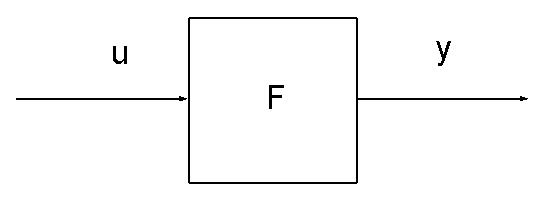
\includegraphics[width = 0.5\textwidth]{./Images/basic_block.eps}
	\caption{Illustration av ett enkelt blockschema.}
	\label{fig:basic_block}
\end{figure}

Med denna figuren menas att $Y(s) = F(s)U(s)$.

\paragraph{Rotort}
En rotort är en plott av ett systems poler som funktion av någon parameter. Den är typiskt uppdelad i grenar, som är kurvor i planet som är parametriserade av parametervärdet. Polerna som motsvarar parametervärdet $0$ är rotortens startpunkter, och polarna motsvarande parametervärdet $\infty$ är rotortens ändpunkter. Om rotorten närmar sig kurvor, är dessa rotortens asymptoter.

\section{Potentialteori}
Potentialteorin som betraktas här är för fall med symmetri i $z$-riktning, tror jag.

\paragraph{Strömfunktionen}
Kontinuitetsekvationen för en inkompressibel fluid ger
\begin{align*}
	\del{x}{u_{x}} + \del{y}{u_{y}} = 0.
\end{align*}
Lösningen av detta ges av strömfunktionen $\Psi$. Den definieras så att
\begin{align*}
	\del{y}{\Psi} = u_{x},\ \del{x}{\Psi} = -u_{y}.
\end{align*}
En viktig karakteristik för strömfunktionen fås genom att betrakta en liten ändring
\begin{align*}
	\dd{\Psi} = \grad{\Psi}\cdot\dd{\vb{r}} = -u_{y}\dd{x} + u_{x}\dd{y}.
\end{align*}
Om vi rör oss längsmed en strömlinje, är denna lilla ändringen lika med $0$.

\paragraph{Potentiallösning för vorticitetsfria fluider}
Om en fluid är vorticitetsfri, gäller det att
\begin{align*}
	\vb{u} = \grad{\Phi}.
\end{align*}
Inkompressibilitetsvillkoret är då
\begin{align*}
	\laplacian{\Phi} = 0.
\end{align*}

\paragraph{Exempel: Potential för strömning kring en cylinder}
I cylinderkoordinater är gradientoperatorn $\grad = \ub{r}\del{r} + \frac{1}{r}\ub{\phi}\del{\phi}$ och laplaceoperatorn $\laplacian = \del[2]{r} + \frac{1}{r}\del{r} + \frac{1}{r^{2}}\del[2]{\phi}$. För att studera strömningen av en inviskös fluid kring en cylinder med radien $a$ centrerad i origo, söker vi då lösningen till
\begin{align*}
	\del[2]{r}{\Phi} + \frac{1}{r}\del{r}{\Phi} + \frac{1}{r^{2}}\del[2]{\phi}{\Phi} = 0,\ \del{r}{\Phi}\eval_{r = a} = 0,\ \left(\ub{r}\del{r}{\Phi} + \frac{1}{r}\ub{\phi}\del{\phi}{\Phi}\right)\eval_{r = \infty} = U\ub{x}.
\end{align*}
Vi löser detta med en separabel ansats - mer specifikt $\Phi = R(r)\cos{\phi}$. För att se att detta är en bra ansats, titta på det andra randvillkoret för $\theta = 0$. Givet detta fås
\begin{align*}
	\cos{\phi}\dv[2]{R}{r} + \frac{\cos{\phi}}{r}\dv{R}{r} - \frac{\cos{\phi}}{r^{2}}R &= 0, \\
	r^{2}\dv[2]{R}{r} + r\dv{R}{r} - R                                                 &= 0.
\end{align*}
Genom att ansätta $R = r^{n}$ för något $n$ fås
\begin{align*}
	(n(n - 1) + n - 1)r^{n} = (n^{2} - 1)r^{n} = 0.
\end{align*}
Om detta skall gälla för alla $r$, måste $n = \pm 1$ och $R = Ar + \frac{B}{r}$. Första randvillkoret ger
\begin{align*}
	A - \frac{B}{a^{2}} = 0,\ R = A\left(r + \frac{a}{r}a\right).
\end{align*}
Andra randvillkoret ger för $\phi = 0$
\begin{align*}
	\left(\ub{r}A\left(1 - \frac{a^{2}}{r^{2}}\right) - \frac{\sin{\phi}}{r}\ub{\phi}A\left(r + \frac{a}{r}a\right)\right)\eval_{\phi = 0,\ r = \infty} = \ub{x}A,
\end{align*}
och den slutgiltiga lösningen är
\begin{align*}
	\Phi = U\cos{\phi}\left(r + \frac{a}{r}a\right).
\end{align*}
Vi noterar till senare att detta kan skrivas
\begin{align*}
	\Phi = U\cos{\phi}r + U\cos(-\phi)\frac{a}{r}a = \Re\left(Uz + \frac{Ua^{2}}{z}\right).
\end{align*}
Hastighetskomponenterna är
\begin{align*}
	u_{r} = U\cos{\phi}\left(1 - \frac{a^{2}}{r^{2}}\right),\ u_{\phi} = -U\sin{\phi}\left(1 + \frac{a^{2}}{r^{2}}\right).
\end{align*}

\paragraph{d'Alemberts paradox}
d'Alemberts paradox är att teorin för potentialströmning ger att luftmotståndet på en godtycklig kropp är $0$. Detta är rimligt eftersom vi inte tar med viskösa effekter, som kommer introduceras.

\paragraph{Komplex potential}
Vi inför nu den komplexa strömfunktionen $W = \Phi + i\Psi$. Om detta ska vara en analytisk funktion (alltså kunna skrivas som en funktion av ett komplext tal $w = x + iy$ så att realdelen och imaginärdelen behandlas likadant), måste den uppfylla Cauchy-Riemanns ekvationer
\begin{align*}
	\del{x}{\Phi} = \del{y}{\Psi},\ \del{y}{\Phi} = -\del{x}{\Psi}.
\end{align*}
Genom att välja realdelen till att vara hastighetsfältets fås att imaginärdelen är strömfunktionen, och motsatt. Cauchy-Riemanns ekvationer implicerar nu direkt att både realdelen och imaginärdelen uppfyller Laplace' ekvation.

\paragraph{Hastighetsfältet från potentialen}
Hastighetsfältet kan beräknas på tre olika sätt:
\begin{itemize}
	\item Beräkna $\dv{W}{w}$ längsmed en vilken som helst riktning. Om man exempelvis fixerar $y$ fås $\dv{W}{w} = u_{x} - iu_{y}$.
	\item Beräkna $\grad{\Re(W)}$.
	\item Beräkna $\curl(\Im(W)\ub{z})$.
\end{itemize}

\paragraph{Potential för friström}
\begin{align*}
	W = Uw.
\end{align*}

\paragraph{Strömning kring ett hörn}
Betrakta funktionen
\begin{align*}
	W = Aw^{n} = Ar^{n}e^{in\theta}
\end{align*}
där $A$ är en konstant och $n > \frac{1}{2}$. Strömlinjerna ges av att imaginärdelen av $W$ är konstant. Två såna, som motsvarar $\Im(W) = 0$, är $\theta = 0$ och $\theta = \frac{\pi}{n}$. Därmed kan detta tolkas som potentialen för strömning kring ett hörn med öppningsvinkel $\frac{\pi}{n}$.

\paragraph{Potential för en källa och en sänka}
Betrakta funktionen
\begin{align*}
	W = \frac{m}{2\pi}\ln{w} = \frac{m}{2\pi}(\ln{r} + i\theta).
\end{align*}
De motsvarande hastighetskomponenterna är
\begin{align*}
	u_{r} = \frac{m}{2\pi r},\ u_{\theta} = 0.
\end{align*}
Flödet ut ur en kurva kring origo ges av
\begin{align*}
	q = \integ{C}{}{l}{u_{r}} = m.
\end{align*}
Tecknet på $m$ ger alltså om det är en källa eller sänka, och beloppet ger styrkan.

\paragraph{Potential för virvel}
Betrakta funktionen
\begin{align*}
	W = \frac{i\Gamma}{2\pi}\ln{w} = \frac{\Gamma}{2\pi}(-\theta + i\ln{r}).
\end{align*}
De motsvarande hastighetskomponenterna är
\begin{align*}
	u_{r} = 0,\ u_{\theta} = -\frac{\Gamma}{2\pi r}.
\end{align*}
Detta är en virvel med cirkulationen $\Gamma$ i medurs riktning.

\paragraph{Dipol}
Betrakta funktionen
\begin{align*}
	W = \frac{\mu}{z}.
\end{align*}
Genom att sätta $\frac{\mu}{2\Im{W}} = -C$ kan man visa att strömlinjerna ges av
\begin{align*}
	x^{2} + (y - C)^{2} = C^{2}.
\end{align*}
Detta är cirklar med radius $C$ och centrum i $(0, C)$, vilket motsvarar strömningar från origo i cirklar som tangerar origo.

\paragraph{Kutta-Jukowskis sats}
Kutta-Jukowskis sats säjer att lyftkraften på en kropp ges av $\rho U\Gamma$, där $\Gamma$ är cirkulationen kring kroppen. Detta är en god approximation för många olika kroppar, speciellt tunna, strömlinjeformade kroppar.

\section{Viskösa fluider}

\paragraph{Töjningstensorn}
Betrakta ett litet fluidelement som rör sig i någon riktning $x_{i}$. Över elementets längd $\cha{x}$ ändras hastigheten med $\del{i}{u_{i}}\cha{x_{i}}$. Över ett litet tidsintervall $\cha{t}$ kommer då fluidelementet att förlängas med $\cha{s} = \del{i}{u_{i}}\cha{x_{i}}\cha{t}$. Den linjära töjningen definieras som förlängningen per längd och tid, och ges här i $x_{i}$-riktningen av $\del{i}{u_{i}}$.

Betrakta vidare ett fluidelement i ett hastighetsfält i $x_{1}x_{2}$-planet. Det kommer skjuvas över en tid $\cha{t}$ så att det bildar en vinkel $\cha{\alpha}$ med $x_{2}$-axeln och $\cha{\beta}$ med $x_{1}$-axeln. Trigonometri ger
\begin{align*}
	\cha{\alpha} = \frac{(u_{1} + \del{2}{u_{1}}\cha{x_{2}} - u_{1})\cha{t}}{\cha{x_{2}}} = \del{2}{u_{1}}\cha{t},\ \cha{\beta} = \del{1}{u_{2}}\cha{t}.
\end{align*}
Skjuvningen per tid ges av $\del{1}{u_{2}} + \del{2}{u_{1}}$.

Vi definierar nu töjningstensorn
\begin{align*}
	e_{ij} = \del{i}{u_{j}} + \del{j}{u_{i}}.
\end{align*}
Från denna kan vi få töjningen av ett givet element.

Vi noterar två saker: Töjningstensorn är symmetrisk, och för inkompressibla vätskor är den spårlös. Som med andra tensorer finns det även ett huvudaxelsystem där töjningstensorn är diagonal.

\paragraph{Friktion i fluider}
Friktion i fluider uppkommer vid töjning. Vi kommer behandla den som om den är proportionell mot töjningen.

\paragraph{Konstitutiva relationer och Newtonska fluider}
För en inkompressibel fluid kommer vi arbeta med den konstitutiva relationen
\begin{align*}
	\tau_{ij} = -p\delta_{ij} + 2\mu e_{ij}.
\end{align*}
En inkompressibel vätska som uppfyller denna konstitutiva relationen kallas för en Newtonsk fluid.

\paragraph{Viskositet}
I relationen ovan införde vi viskositeten $\mu$.

\paragraph{Navier-Stokes' ekvation för en Newtonsk fluid}.
Vi har
\begin{align*}
	\del{j}{\tau_{ij}} = -\del{i}{p} + \mu(\del{j}{\del{j}{u_{i}}} + \del{j}{\del{i}{u_{j}}}).
\end{align*}
Genom att ordna om derivatorna innehåller den sista termen en derivata av hastighetsfältets divergens. Eftersom vi studerar Newtonska fluider är denna $0$, och
\begin{align*}
	\del{j}{\tau_{ij}} = -\del{i}{p} + \mu\del{j}{\del{j}{u_{i}}}.
\end{align*}
Vi inför nu kinematiska ekvationen $\nu = \frac{\mu}{\rho}$, och skriver då kraftekvationen som
\begin{align*}
	\mdv{u_{i}} = -\frac{1}{\rho}\del{i}{p} + \nu\del{j}{\del{j}{u_{i}}} + g_{i}.
\end{align*}
Detta är Navier-Stokes' ekvation(er) för en Newtonsk fluid. På vektorform är den
\begin{align*}
	\del{t}{\vb{u}} + (\vb{u}\cdot\grad)\vb{u} = -\frac{1}{\rho}\grad{p} + \nu\laplacian{\vb{u}} + \vb{g}.
\end{align*}

Eftersom det finns friktion i vätskan, har ekvationen som randvillkor att $\vb{u} = \vb{0}$ på fasta ränder, eftersom vätskan kommer röra sig med randen.

\paragraph{Förenkling genom borttagning av kraftterm}
Antag att gravitationen inte driver flödet av en vätska utan bara sätter upp ett tryckfält i vätskan, och att detta är enda yttre kraften på vätskan. Då kan vi skriva $p = p' + p_{g}$, där $p_{g}$ är trycket som uppstår på grund av gravitationen. Denna termen uppfyller $\rho\vb{g} - \grad{p_{g}} = 0$. Då blir Navier-Stokes' ekvation
\begin{align*}
	\del{t}{\vb{u}} + (\vb{u}\cdot\grad)\vb{u} = -\frac{1}{\rho}\grad{p'} + \nu\laplacian{\vb{u}}.
\end{align*}
Primmet tas oftast ej med.

\section{Lösningar av Navier-Stokes' ekvation för newtonska fluider}

Detta är lösningar av Navier-Stokes' ekvation för newtonska fluider i vissa specifika geometrier.

\paragraph{Couetteströmning}
Betrakta en fluid mellan två plattor. Fluiden har kinematisk viskositet $\nu$, täthet $\rho$, konstant tryck $p$ och befinner sig långt från in- och utlopp (vi säjer att strömningen är fullt utbildad). Plattorna är på ett avstånd $h$ i $y$-riktning. Ena plattan är fäst, och andra plattan rör sig med en hastighet $U$ i $x$-riktning. Vi vill nu bestämma stationära hastighetsfältet, volymsflödet per enhet längd i $z$-riktning och spänningen på de två plattorna.

Vi noterar först att problemet är symmetriskt i både $x$ och $z$. Eftersom det inte finns något som driver flöde i $z$-riktning, måste $u_{z} = 0$. Då ger inkompressibilitetsvillkoret att $u_{y}$ är konstant och lika med $0$ för att uppfylla randvillkoret. Det som återstår av Navier-Stokes' ekvation är
\begin{align*}
	\laplacian{u_{x}} = \del[2]{y}{u_{x}} = 0,
\end{align*}
och slutligen
\begin{align*}
	u_{x} = U\frac{y}{h}.
\end{align*}

Volymsflödet per längdenhet ges av
\begin{align*}
	\Phi = \frac{1}{l}\vinteg{x = c}{}{S}{\vb{u}} = \frac{1}{l}\integ{0}{l}{z}{\integ{0}{h}{y}{U\frac{y}{h}}} = \frac{1}{2}Uh.
\end{align*}

För att hitta spänningarna längsmed ytorna, konstaterar vi först att ytorna har normalvektor $n_{i} = \pm\delta_{i2}$. Ytspänningarna ges då av
\begin{align*}
	\tau_{ij}n_{j} = \pm\tau_{i2} = \pm\mu(\del{i}{u_{2}} + \del{2}{u_{i}}).
\end{align*}
Den enda nollskilda kraftkomponenten är den första, och ges av
\begin{align*}
	f_{1} = \tau_{1j}n_{j} = \pm\mu\frac{U}{h} = \pm\frac{\rho\nu U}{h}.
\end{align*}

\paragraph{Poiseuille-strömning}
Betrakta en fluid mellan två plattor. Fluiden har kinematisk viskositet $\nu$, täthet $\rho$, tryck $p$ med konstant gradient $-K\ub{x}$ och strömningen är stationär och fullt utbildad. Plattorna är båda fästa på ett avstånd $h$ i $y$-riktning. Vi vill nu bestämma stationära hastighetsfältet, volymsflödet per längdenhet i $z$-riktning och spänningen på de två plattorna.

På samma sätt som för Couetteströmning fås $u_{y} = u_{z} = 0$ och symmetri i $x$ och $z$. Navier-Stokesä ekvation ger då
\begin{align*}
	\nu\laplacian{u_{x}} = \nu\del[2]{y}{u_{x}} = \frac{1}{\rho}\ub{x}\del{x}{p} = -\frac{K}{\rho},\ \del[2]{y}{u_{x}} = -\frac{K}{\mu}.
\end{align*}
Detta har lösning
\begin{align*}
	u_{x} = \frac{1}{2}\frac{Kh^{2}}{\mu}\left(\frac{y}{h} - \left(\frac{y}{h}\right)^{2}\right).
\end{align*}

Volymsflödet per längdenhet ges av
\begin{align*}
	\Phi &= \frac{1}{l}\vinteg{x = c}{}{S}{\vb{u}} \\
	     &= \frac{1}{l}\integ{0}{l}{z}{\integ{0}{h}{y}{\frac{1}{2}\frac{Kh^{2}}{\mu}\left(\frac{y}{h} - \left(\frac{y}{h}\right)^{2}\right)}} \\
	     &= \frac{1}{2}\frac{Kh^{3}}{\mu}\integ{0}{1}{u}{(u - u^{2})} \\
	     &= \frac{1}{12}\frac{Kh^{3}}{\mu}.
\end{align*}

Normalvektorn ges på samma sätt som innan, och vi får
\begin{align*}
	\tau_{ij}n_{j} = \pm\mu(\del{i}{u_{2}} + \del{2}{u_{i}}).
\end{align*}
Enda nollskilda komponenten är
\begin{align*}
	f_{1} = \pm\frac{1}{2}Kh\left(1 - 2\frac{y}{h}\right).
\end{align*}
Denna är lika med $\frac{1}{2}Kh$ på båda ytorna.

\paragraph{Stokes' första problem}
Betrakta en newtonsk fluid med kinematisk viskositet $\nu$ och täthet $\rho$ i det halvoändliga rummet $y > 0$. Vid randen börjar en platta röra sig med hastighet $U$ i $x$-riktningen vid $t = 0$. Vi vill nu bestämma hastighetsfältet.

Systemet är symmetriskt i $xz$-planet, och inkompressibiliteten ger då $\del{y}{u_{y}} = 0$. För att uppfylla randvillkoret måste då $u_{y} = 0$. Återigen finns det inget som driver flöde i $z$-riktning, så $u_{z} = 0$. Navier-Stokes' ekvation ger då
\begin{align*}
	\del{t}{u_{x}} = -\frac{1}{\rho}\del{x}{p} + \nu\laplacian{u_{x}}.
\end{align*}
Återigen använder vi symmetrin för att skriva detta som
\begin{align*}
	\del{t}{u_{x}} = \nu\del[2]{y}{u_{x}}.
\end{align*}
Vi kommer lösa detta med en likformighetsansats med den dimensionslösa variabeln $\eta = \frac{y}{\sqrt{\nu t}}$ på formen
\begin{align*}
	u_{x} = Uf(\eta).
\end{align*}
Jag borde lösa klart det här någon gång.

\section{Viskösa effekter}

\paragraph{Bildningen av gränsskikt}
Vidhäftningsvillkoret gör att nära ytor ändras hastigheten extremt snabbt i ett tunt skikt nära ytan, det så kallade gränsskiktet. Vi kommer studera beteendet i och utanför såna gränsskikt i fall som är symmetriska i $z$-riktning.

\paragraph{Formulering av problem}
Vi kommer betrakta strömning av en fluid i $x$-riktning med friströmshastighet $U$. Fluiden strömmar förbi en platta som är parallell med $x$-riktningen och har längd $L$. Över ytan finns ett gränsskikt med tjocklek $\delta$

\paragraph{Reynoldstalet}
Navier-Stokes' ekvation ger
\begin{align*}
	u_{x}\del{x}{u_{x}} + u_{y}\del{y}{u_{x}} = -\frac{1}{\rho}\del{x}{p} + \nu(\del[2]{x}{u_{x}} + \del[2]{y}{u_{x}}).
\end{align*}
Vi studerar först problemet i gränsskiktet. Här är viskösa krafter viktiga, så $y$-derivatan kommer vara stor här. Om vi av någon oklar anledning antar att $x$-derivatan är av ledande ordning på vänstersidan, blir detta
\begin{align*}
	u_{x}\del{x}{u_{x}} = \nu\del[2]{y}{u_{x}}.
\end{align*}
Detta låter oss göra en grov storleksuppskattning
\begin{align*}
	\frac{U^{2}}{L} = \nu\frac{U}{\delta^{2}},\ \frac{\delta}{L} = \frac{1}{\sqrt{\rey}},
\end{align*}
där $\rey = \frac{UL}{\nu}$ är Reynoldstalet. I de flesta tillämpningar är Reynoldstalet stort, så gränsskiktet är tunt.

\paragraph{Dimensionslösa variabler}
Vi vill nu förenkla Navier-Stokes' ekvationer för stora Reynoldstal. För att göra detta låter vi $U$ och $p_{\infty}$ vara hastigheten och trycket långt uppströms. Vi antar att $u_{x}$ är av storleksordning $U$ och att $\del{x}{p} = \rho u_{x}\del{x}{u_{x}}$. Detta ger storleksordningsuppskattningen
\begin{align*}
	p_{\infty} - p \approx \rho U^{2}.
\end{align*}
Vi kan även skatta vertikala hastigheten med hjälp av inkompressibilitetsvillkoret som
\begin{align*}
	u_{y} \approx \frac{\delta}{L}U = \frac{1}{\sqrt{\rey}}U.
\end{align*}
Detta motiverar oss att införa de dimensionslösa variablerna
\begin{align*}
	x' = \frac{x}{L},\ y' = \frac{y}{\delta} = \sqrt{\rey}\frac{y}{L},\ u_{x}' = \frac{u_{x}}{U},\ u_{y}' = \sqrt{\rey}\frac{u_{y}}{U},\ p' = \frac{p_{\infty} - p}{\rho U^{2}}.
\end{align*}
I termer av dessa variabler är Navier-Stokes' ekvationer
\begin{align*}
	u_{x}'\del{x'}{u_{x}'} + u_{y}'\del{y'}{u_{x}'}                 &= -\del{y'}{p'} + \frac{1}{\rey}\del[2]{x'}{u_{x}'} + \del[2]{y'}{u_{x}'}, \\
	\frac{1}{\rey}(u_{x}'\del{x'}{u_{y}'} + u_{y}'\del{y'}{u_{y}'}) &= -\del{y'}{p'} + \frac{1}{\rey^{2}}\del[2]{x'}{u_{x}'} + \frac{1}{\rey}\del[2]{y'}{u_{x}'}, \\
	\del{x'}{u_{x}'} + \del{y'}{u_{y}'} = 0.
\end{align*}
För stora Reynoldstal kan vi nu bortse från många termer här. I våra ursprungliga variabler fås då
\begin{align*}
	u_{x}\del{x}{u_{x}} + u_{y}\del{y}{u_{x}}                 &= -\del{y}{p} + \del[2]{y}{u_{x}}, \\
	0                                                         &= -\del{y}{p}, \\
	\del{x}{u_{x}} + \del{y}{u_{y}} = 0.
\end{align*}
Man kan tydligen även använda Bernoullis ekvation (fast inte) längsmed en strömlinje som följer gränsskiktets rand. Vi får då
\begin{align*}
	\frac{p}{\rho} + \frac{1}{2}U^{2} = c,\ -\frac{1}{\rho}\del{x}{p} = U\del{x}{U}.
\end{align*}
Nu har vi ställt upp alla ekvationer, och vi har randvillkoren
\begin{align*}
	u_{x}(x, 0) = u_{y}(x, 0) = 0,\ u_{x}(x, \infty) = U,
\end{align*}

\paragraph{Mått på tjocklek}
Härifrån måste vi välja någon definition av gränsskiktets tjocklek. Detta är tre olika sätt att göra det på.

\paragraph{Delta-nittinio}
Delta-nittinio-måttet definieras av
\begin{align*}
	u(x, \delta_{99}) = 0.99U.
\end{align*}

\paragraph{Förträngningstjockleken}
Förträngningstjockleken definieras som avståndet i vertikal riktning en strömlinje långt från väggen förflyttas på grund av väggen.

För att beräkna den observerar vi att masskonserveringen ger
\begin{align*}
	\integ{0}{h}{y}{U} = \integ{0}{h + \delta_{\star}}{y}{u_{x}},
\end{align*}
där vi gör andra integralen på ett (långt?) avstånd från där strömningen möter plattan. Eftersom vi pratar om strömlinjer långt från väggen, gör vi skattningen $u_{x} = U$ långt borta, vilket ger
\begin{align*}
	\delta_{\star} = \integ{0}{h}{y}{1 - \frac{u_{x}}{U}}.
\end{align*}

\paragraph{Rörelsemängdtjocklek}
Om tryckgradienten är noll fås för kontrollvolymen vi studerade ovan
\begin{align*}
	-f = -\integ{0}{h}{y}{\rho U^{2}} + \integ{0}{h + \delta_{\star}}{y}{\rho u_{x}^{2}}
\end{align*}
där
\begin{align*}
	f = \integ{0}{x}{x}{\mu\del{y}{u_{x}}(x, 0)}
\end{align*}
är friktionskraften i $x$-riktning på den delen av plattan som är innanför kontrollvolymen. Vi definierar nu rörelsemängdstjockleken
\begin{align*}
	\theta &= \frac{f}{\rho U^{2}} \\
	       &= \integ{0}{h}{y}{1 - \left(\frac{u_{x}}{U}\right)^{2}} + \frac{1}{U^{2}}\integ{h}{h + \delta_{\star}}{y}{u_{x}^{2}} \\
	       &\approx \integ{0}{h}{y}{1 - \left(\frac{u_{x}}{U}\right)^{2}} + \delta_{\star} \\
	       &= \integ{0}{h}{y}{\frac{u_{x}}{U}\left( 1 - \frac{u_{x}}{U}\right)}.
\end{align*}
Vi kan tydligen skriva detta som
\begin{align*}
	\theta = \integ{0}{\infty}{y}{\frac{u_{x}}{U}\left( 1 - \frac{u_{x}}{U}\right)}.
\end{align*}

\paragraph{Blasius' gränsskikt}
Blasius' lösning för gränsskiktet är en något annorlunda lösning av samma problemet vi har studerat. I detta fall är tryckgradienten lika med noll och strömningen möter plattan i origo. Inkompressibilitetsvillkoret låter oss införa strömfunktionen $\Psi$, och Navier-Stokes' ekvationer ger
\begin{align*}
	\del{y}{\Psi}\del{y}{\del{x}{\Psi}} - \del{x}{\Psi}\del[2]{y}{\Psi} = \nu\del[3]{y}{\Psi}.
\end{align*}
Eftersom systemet ej ändras under addition av en konstant till strömfunktionen, kan vi välja $\Psi(x, 0) = 0$. De övriga randvillkoren blir
\begin{align*}
	\del{y}{\Psi}(x, 0) = 0,\ \del{y}{\Psi}(x, y) \to U.
\end{align*}
Vi kommer lösa detta problemet med en likformighetsansats
\begin{align*}
	u_{x} = Uf'(\eta),\ \eta = \frac{y}{\delta(x)}.
\end{align*}
Detta ger
\begin{align*}
	\Psi = \integ{0}{y}{y}{u_{x}} = U\delta\integ{0}{\eta}{\eta}{f'(\eta)} = U\delta f(\eta).
\end{align*}
Insatt i Navier-Stokes' ekvation ger detta
\begin{align*}
	f''' = -\left(\frac{U\delta}{\nu}\dv{\delta}{x}\right)ff''.
\end{align*}
Om detta skall gälla, måste prefaktorn vara en konstant. Vi kan sätta den till $\frac{1}{2}$, vilket ger
\begin{align*}
	\delta = \sqrt{\frac{\nu x}{U}}.
\end{align*}
Att ändra den konstanten skulle bara motsvara en omskalning av enheterna, så vi ser att valet av konstant är godtyckligt. Den återstående ekvationen är
\begin{align*}
	\frac{1}{2}ff'' + f''' = 0,
\end{align*}
med randvillkor
\begin{align*}
	f(0) = 0,\ f'(0) = 0,\ f'(\eta) \to 1.
\end{align*}

Vi kan även beräkna väggskjuvspänningen
\begin{align*}
	\tau = \mu\del{y}{u_{x}}(x, 0) = \frac{0.332\rho U^{2}}{\sqrt{\rey_{x}}}
\end{align*}
där $\rey_{x}$ är Reynoldstalet beräknad med $x$. Det totala aerodynamiska moståndet på plattan ges då av
\begin{align*}
	F = \integ{0}{L}{x}{\tau} = \frac{0.664\rho U^{2}}{\sqrt{\rey_{L}}}.
\end{align*}
Vi kan även definiera en motståndskoefficient
\begin{align*}
	C = \frac{F}{\frac{1}{2}\rho U^{2}} = \frac{1.33}{\sqrt{\rey_{L}}}.
\end{align*}

\paragraph{Avlösning}
Kring kroppar som omges av strömning kommer det bildas gränsskikt där vorticiteten är hög. Detta kommer påverka strömningen med olik karaktär beroende på ett Reynoldstal som beskriver strömningen.

\paragraph{Motståndskraft på kropp i fluid}
Betrakta en statisk kropp i en fluid med friströmshastighet $U\ub{x}$. På denna är motståndskraften
\begin{align*}
	F = \frac{1}{2}C_{D}\rho U^{2}S
\end{align*}
där $S$ är den projicerade arean i strömriktningen och $C_{D}$ är en motståndskoefficient som beror på Reynoldstalet.

\end{document}
